\section{Diagramma entità-relazione}\label{sec:conceptdiagram}
Il {\it diagramma concettuale} finale è mostrato \vpageref{diagram.1}.

%Si noti che si è deciso di aggiungere una {\it ridondanza} nell'entità {\tt Comanda}:
%l'attributo {\tt Stato} della comanda può infatti essere determinato dallo stato di
%tutti i piatti ordinati nella comanda. Decidiamo però di mantenere tale ridondanza:
%il motivo di questa decisione sarà discusso nel \vref{ch:redundancies}.

La spiegazione di come sono stati realizzati il {\it procedimento strutturato} e le {\it variazioni}
(e quindi anche i {\it suggerimenti}) è disponibile nel paragrafo \vref{sec:structuredprocess}.
\clearpage
\newgeometry{margin=2cm}
\thispagestyle{plain}
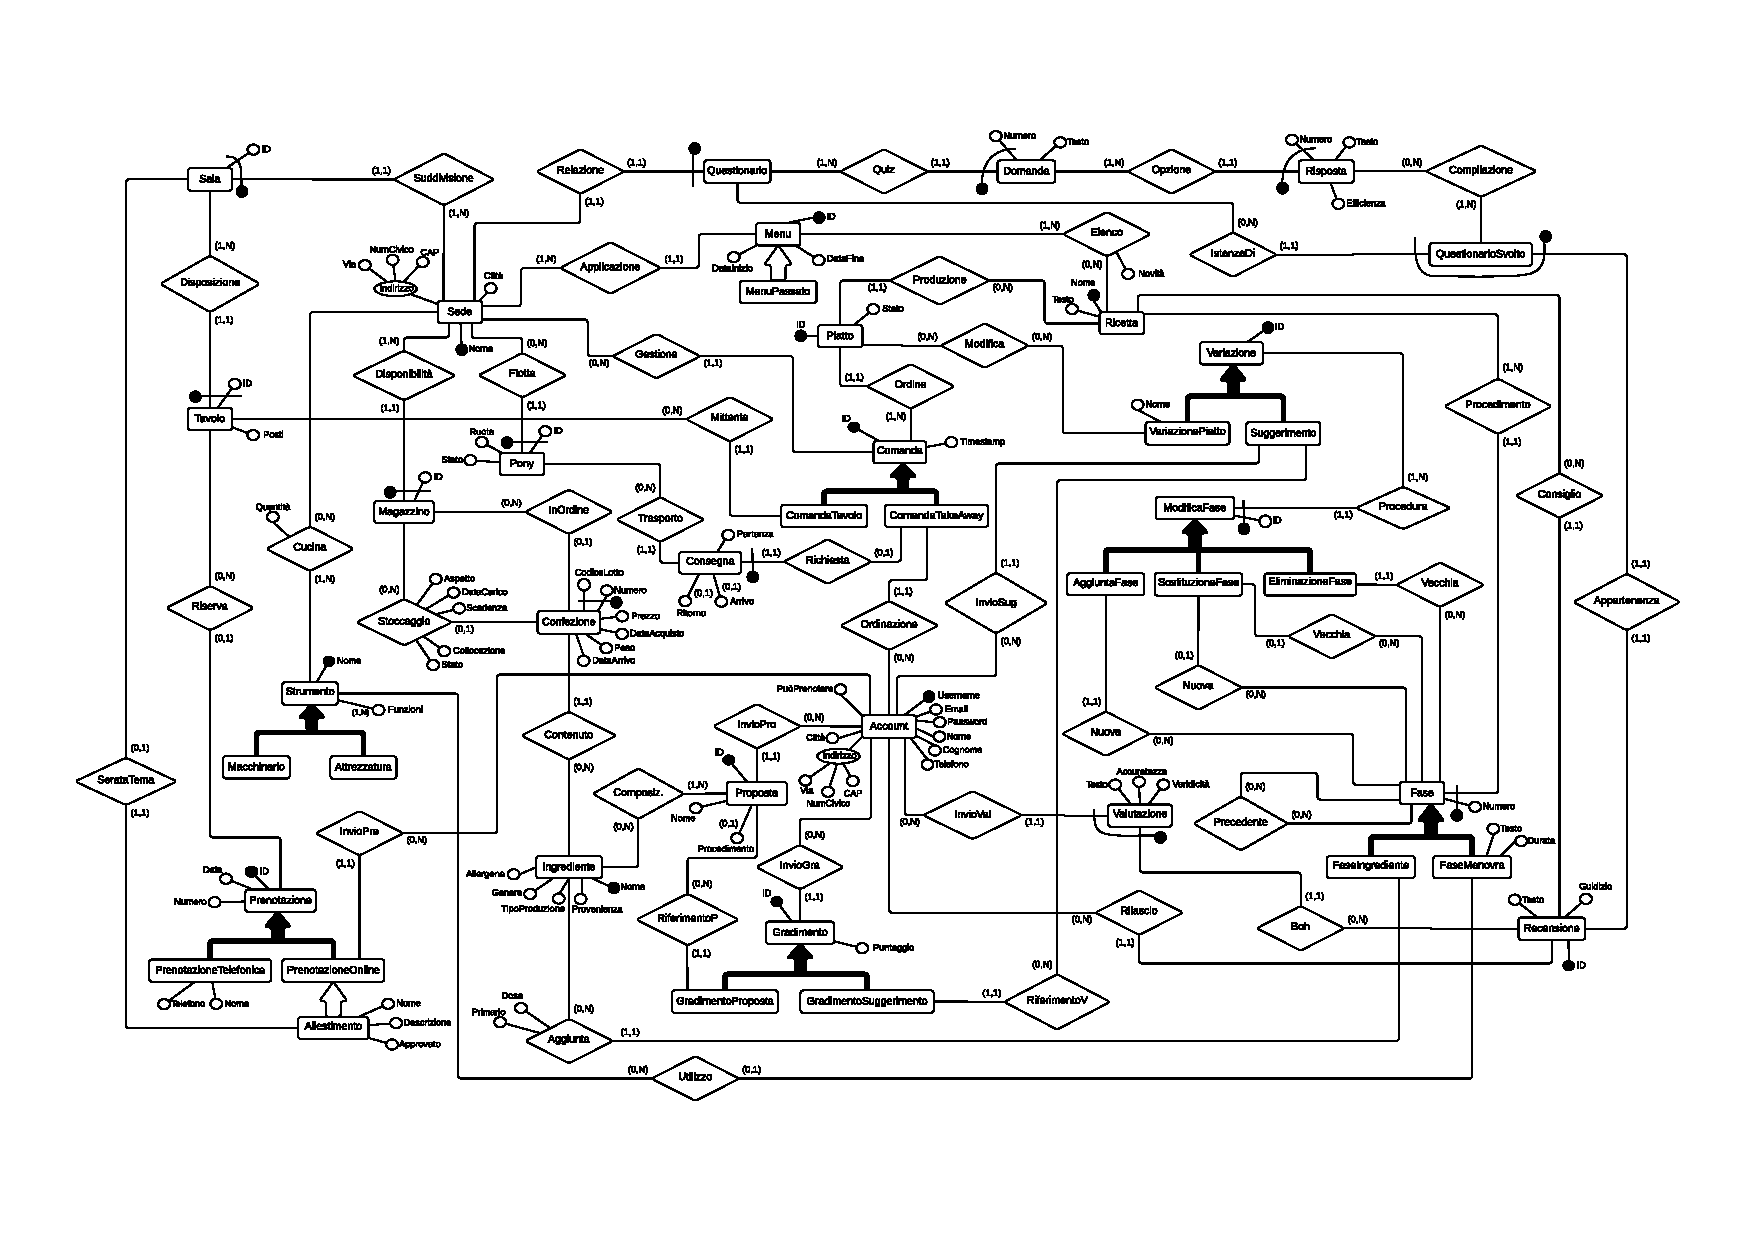
\includepdf[pages={1},landscape=true,pagecommand={\refstepcounter{includepdfpage}\label{diagram.\theincludepdfpage}}]{./images/diagrams.pdf}
\restoregeometry
